\documentclass[crop,tikz]{standalone}

\usepackage{xcolor}
\usepackage{tikz}
\usetikzlibrary{automata, positioning, calc, shapes, arrows, fit}
\newcommand{\mycircle}{\resizebox{!}{0.7em}{\tikz[baseline=(char.base)]{
	\node[shape=circle, fill={rgb:red,0;green,3;blue,8}] (char) {};}}}
\newcommand{\myrectangle}{\resizebox{!}{0.7em}{\tikz[baseline=(char.base)]{
	\node[shape=rectangle, fill={rgb:red,0;green,7;blue,6}] (char) {};}}}
\newcommand{\mydiamond}{\resizebox{!}{0.7em}{\tikz[baseline=(char.base)]{
	\node[shape=diamond, fill={rgb:red,0;green,10;blue,5}] (char) {};}}}

\begin{document}
	
% ============= SOC =============
%\begin{tikzpicture}[node distance = 0.2em and 1em]
%\node[] (a1) {$\mycircle$};
%\node[right = of a1] (b1) {$\succ$};
%\node[right = of b1] (c1) {$\myrectangle$};
%\node[right = of c1] (d1) {$\succ$};
%\node[right = of d1] (e1) {$\mydiamond$};
%
%\node[below = of a1] (a2) {$\mydiamond$};
%\node[right = of a2] (b2) {$\succ$};
%\node[right = of b2] (c2) {$\myrectangle$};
%\node[right = of c2] (d2) {$\succ$};
%\node[right = of d2] (e2) {$\mycircle$};
%
%\node[below = of a2] (a3) {$\myrectangle$};
%\node[right = of a3] (b3) {$\succ$};
%\node[right = of b3] (c3) {$\mycircle$};
%\node[right = of c3] (d3) {$\succ$};
%\node[right = of d3] (e3) {$\mydiamond$};
%\end{tikzpicture}

% ============= SOI =============
%\begin{tikzpicture}[node distance = 0.2em and 1em]
%\node[] (a1) {$\mycircle$};
%\node[right = of a1] (b1) {$\succ$};
%\node[right = of b1] (c1) {$\myrectangle$};
%\node[right = of c1] (d1) {$\succ$};
%\node[right = of d1] (e1) {$\mydiamond$};
%
%\node[below = of a1] (a2) {$\mydiamond$};
%\node[right = of a2] (b2) {$\succ$};
%\node[right = of b2] (c2) {$\myrectangle$};
%
%\node[below = of a2] (a3) {$\myrectangle$};
%\node[right = of a3] (b3) {$\succ$};
%\node[right = of b3] (c3) {$\mycircle$};
%\node[right = of c3] (d3) {$\succ$};
%\node[right = of d3] (e3) {$\mydiamond$};
%\end{tikzpicture}

% ============= TOC =============
%\begin{tikzpicture}[node distance = 0.6em and 1em]
%\node[] (a1) {$\mycircle$};
%\node[right = of a1] (b1) {$\succ$};
%\node[right = of b1] (c1) {$\myrectangle$};
%\node[right = of c1] (d1) {$\succ$};
%\node[right = of d1] (e1) {$\mydiamond$};
%
%\node[below = of a1] (a2) {$\mydiamond$};
%\node[right = of a2] (b2) {$\succ$};
%\node[right = of b2, align = center] (c2) {$\myrectangle{}$\\ $\mycircle{}$};
%
%\node[below = of a2] (a3) {$\myrectangle$};
%\node[right = of a3] (b3) {$\succ$};
%\node[right = of b3] (c3) {$\mycircle$};
%\node[right = of c3] (d3) {$\succ$};
%\node[right = of d3] (e3) {$\mydiamond$};
%\end{tikzpicture}

% ============= TOI =============
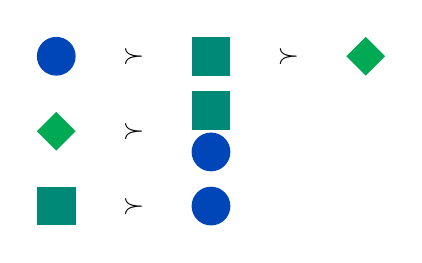
\begin{tikzpicture}[node distance = 0.6em and 1em]
\node[] (a1) {$\mycircle$};
\node[right = of a1] (b1) {$\succ$};
\node[right = of b1] (c1) {$\myrectangle$};
\node[right = of c1] (d1) {$\succ$};
\node[right = of d1] (e1) {$\mydiamond$};

\node[below = of a1] (a2) {$\mydiamond$};
\node[right = of a2] (b2) {$\succ$};
\node[right = of b2, align = center] (c2) {$\myrectangle{}$\\ $\mycircle{}$};

\node[below = of a2] (a3) {$\myrectangle$};
\node[right = of a3] (b3) {$\succ$};
\node[right = of b3] (c3) {$\mycircle$};
\end{tikzpicture}
\end{document}